% Modelling infectious disease dynamics towards informed public-health interventions, with application on \textsc{covid}-19 and cholera.
\chapter*{Introduction} \addcontentsline{toc}{chapter}{Introduction}\markboth{Introduction}{}

 \section{Context}
 Centuries after the first cholera pandemics and 160 years after the realisation that safe drinking-water and adequate sanitation prevent its transmission, cholera remains a threat to millions living in hotspots or at risk areas. And the recent emergence of the new coronavirus disease 2019, \textsc{covid}-19, and the strain it put on world's most advanced healthcare systems recalls the constant risks posed by emerging diseases. 
 
 Public-health policies have proven the effectiveness of interventions against infectious diseases, showing that many deaths are preventable, and in some cases elimination is possible. In the fight against infectious diseases, a serie of successes -- attributable to \eg hygiene, vaccines, antibiotics, safe water, ... -- brough the hope of a global and durable reduction of the burden. Especially in privileged communities, long-term improvements have been achieved for many of the diseases that have shaped the history of humanity. While these progresses show that infectious diseases are not a necessary fate, setbacks on the control of existing and emerging pathogens remind us the ongoing threat they poses on public-health. 
  Indeed, the current global health picture is marked by inequalities in the distribution of the burden, which disproportionaly piles up on already impoverished communities, in conflict zone or after natural disasters. Today, communicable diseases cause approx. 15\% of global deaths every year\cite[-4\baselineskip][tab. 1, excl. non-transmissible neonatal and maternal diseases and nutritional diseases; pre-\textsc{covid}-19 estimates]{Roth:GlobalRegionalNational:2018}, and nearly 1/3 of all child deaths are caused by pneumonia and diarrhoea alone\cite[][\ie 2\textsc{m} deaths among under 5, every year.]{WHO:EndingPreventableChild:2013}.  
  
  As a consequence of the \textsc{covid}-19 pandemic, the present thesis happens to associate two antipodean diseases. Cholera, one of the most ancient recorded disease\footnote[][]{History of pre-pandemic cholera is uncertain but numerous accounts of the disease are supposed from as early as 400\textsc{bce}. See \fullcite[p. 95]{Byrne:EncyclopediaPestilencePandemics:2008}.}, has caused 7 pandemics in the modern era. In contrast, \textsc{covid}-19 earliest known onset of symptoms is on December 1, 2019. The pathogen for cholera is a bacteria, \textit{Vibrio Cholerae}, responsible for heavy watery diarrhea, whereas \textsc{SARS-CoV-2}, \textsc{covid}-19’s pathogen, is a virus responsible for respiratory infections. Cholera belongs to the negletected tropical diseases, a class of understudied infections while the \textsc{covid}-19 pandemic has sparked an unprecedented accumulation of evidence\sidenote[][]{With more than 190'000 peer-reviewed papers and many more preprints, website and reports published at the time of writing. Estimation from: \fullcite{COVID-19OpenAccessProject:LivingEvidenceCOVID19:2020}}. 
Other differences between the two diseases include the posited transmission routes (fecal-oral vs. respiratory) and the affected communities (``poorest of the poor”, higher severity on children vs. global, higher severity on elders). Despite these differences, cholera and \textsc{covid}-19 shares a burden that echoes unequal access to care, disproportionately affecting stigmatized communities, and  mechanisms that makes their transmission sustainable in populations and causes pandemics with a regretfully high toll on human lives. Both cholera and \textsc{covid}-19 are infectious diseases -- with the potential of starting epidemics and pandemics.%, and the many of the scientific methods to study the spread and interventions are shared across these diseases and others.

 
Epidemics -- the rapid spread of an infectious disease in a population -- are  complex phenomena resulting from the interactions between pathogens, environment, societies and individuals\cite{Rinaldo:RiverNetworksEcological:2020a, Buckee:ThinkingClearlySocial:2021, Heesterbeek:ModelingInfectiousDisease:2015}. The mitigation of the spread of infectious disease epidemics presents challenges accross every dimensions of environmental and human health; in order to prevent spillover events, to block transmission routes, and to protect or treat every person appropriatelly. %Public-health policies strive to save lives by designing effective mitigation measures.
 One of the challenges of designing effective public-health policies is dealing with the uncertainties that plague every facet of disease transmission. Only biased and sometime scarce information is available to reason on complex systems with multi-factorial interactions. 
 
%Models are conceptual representations that guide our reasoning about the world.
Models -- conceptual representations of systems -- are tools for us to reason about the world. Historically, conceptual models of the propagation of diseases, from divine retribution to miasma theory, has motivated more (quarantine) or less (persecution) effective approaches to the control of these pests. Scientific breakthroughs in biology and medicine, with the identification of pathogens and their transmission routes, provided a new look on transmission and opened the path for improved preventive interventions and treatments. Novel statistical modeling approaches\cite[-3\baselineskip]{Freedman:AssociationCausationRemarks:1999} developed in the 20th century -- and continuously improved ever since\cite{Gelman:WhatAreMost:2021} --  provide a formal framework to reasons about the propagation of a disease in a population. Models enable one to deal with biases on data collection, to account for epistemic uncertainties, to encompass uncertainties in the transmission dynamics. It becomes possible to simulate the disease spread in the affected populations and to study the impact of intervention policies in a principled way. The toolbox was further re-enforced by advances in mechanistic modeling applied to disease transmission, starting from SIR compartmental models\cite{Kermack:ContributionMathematicalTheory:1927, Anderson:PopulationBiologyInfectious:1979}, which divide the population depending on their status with respect to the disease. And recent advances in computing power proved a paradigm shift in dealing with the available evidence to accurately simulate complex systems.



\section{Modeling infectious diseases}
The present thesis explores compartmental models as an approach to infectious disease transmission, and as tools to guide intervention strategies. In each of the presented research works, it is strove to answer a series of research questions, all being variations of: how do infectious diseases spread ? and how can we prevent them from spreading ? These questions are answered using extensively computer-age modeling and inference methods, in a interactive process represented in fig.~\ref{fig:modeling}. Given a question and information in the form of observations (data) and knowledge, statistical inference is performed in four steps:

\paragraph{Model design} One or more model(s) of disease transmission are designed. Choices on what to include and how to express the supposed dynamics depends on the underlying knowledge of the processes and the available data. An epidemiological model considers a subset of the known transmission processes that are relevant to answer the research or policy questions\footnote[][]{“Since all models are wrong the scientist must be alert to what is importantly wrong. It is inappropriate to be concerned about mice when there are tigers abroad.” from \fullcite{Box:ScienceStatistics:1976}.}. A set of 5 models, see tab.~\ref{tab:allmodels}, is proposed in this thesis, with features that depends on the disease, the context, the possible control measures and the uncertainties associated with the observations and the processes by itself. Some models have stochastic transitions while others are mostly deterministic, some models consider human mobility as fluxes between regions whereas others assume well-mixed population. Despite the foregoing differences, all the models presented in this thesis are compartmental with some mechanistic components\footnote{The opposite would be empirical models, which aim at reproducing observations rather than the relationship between the parts of the system modeled.}; all are based on the SIR model. It means that individuals are caraterized by their status with respect to the disease. In a population some individuals start susceptible $S$ to the disease and might become infected and infectious $I$. After some time they turn recovered $R$: they are immune to infection and do not contribute to transmission anymore. %The infection probability (transition from $S$ to $I$) is called the \textit{force of infection}, and mass action
Additional compartments may be defined depending on the objective of the exercise. In tab.~\ref{tab:allmodels}, the principal compartments of the considered models are indicated: exposed $E$ (incubating, infectious or not), asymptomatic $A$ (infectious with no symptoms), $H$ indicate compartments that represent the healthcare facilities (hospitalisation, ICUs), $V$ the compartments for vaccinated individuals, and finally $B$ the modeling of an environmental bacteria reservoir for cholera models\footnote{In this table, the exponents denote the number of sub-compartments of the same type used to model non-exponential distributions of the residence times in that compartment, using the linear-chain trick.}.
In these models, some states are observed through a reporting process (\eg infected $I$ may be reported as incident cases), but most most are unobserved. Likewise some parameters are fixed to values (or distribution of values) that are known more or less precisely, while many others are left unknown.

 \begin{figure*}\centering
  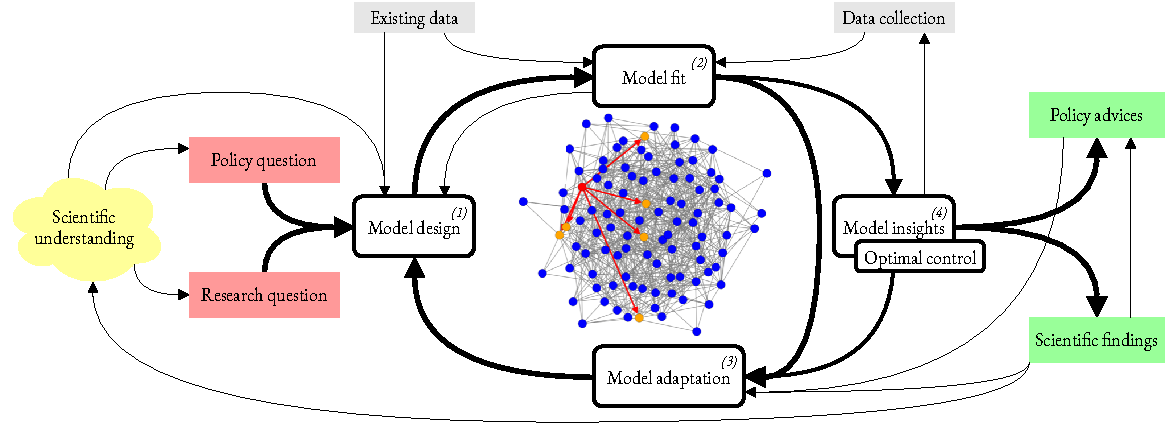
\includegraphics{fig/modeling_cycle}
  \caption[Processes for infectious disease modeling][-1\baselineskip]{Processes for  infectious disease modeling. The numerous feedback loops makes this procedure iterative. All boxes save for data collection were explored in this thesis. The central figure represents an agent-based model of disease transmission in a random graph (by Thomas Fry, a master student supervised during this thesis, with permission).}\label{fig:modeling}
\end{figure*}
\paragraph{Model fit} \textit{Fitting} conditions the model on the observed data. It allows to infer unobserved states and parameters from reported quantities, such as the reduction of transmission during lockdown from hospitalization and deaths. A panel of methods for fitting a model to data has been developed. Usually computer-age statistical inference relies on thousands of model simulations to explore the high dimensionals parameter and state spaces; each realisation being evaluated against the data. The inner working of the fitting algorithms varies depending on formal framework it is built on, but also on the numerous computational tricks to make inference fast and precise. In this thesis, two classes of methods are used: bayesian methods based on Markov chain Monte Carlo (MCMC) derivatives and frequentist Iterated Filtering (IF) methods. Fitting the model allows one to uncover previously unknown transmission parameters and unobservable states. As such, it requires a high-degree of care as infered features may be caused by modeling artifacts instead of real epidemic features. Moreover results may misrepresent the uncertainties associated with the process. As these methods fail more or less gracefully, it is possible to obtain results that are both confident and wrong.
 
\paragraph{Model adaptation} An evaluation of the \textit{fit} of the model and the implication on the results is done by performing visuals and formal checks. More often than not it is necessary to adapt either the fitting procedure or the model structure. It could be the inclusion or the removal of a process from the model. Or perhaps choosing to account for dynamics in a more or less explicit, detailled way. Models are lossy compressions of reality (from an information theory point of view), and choices on the processes to be included, and how to include them are the cornerstone of epidemiological modeling. Indeed despite its recent formalism, statistical inference remains an art, uncomfortably dependent on the practitioners, their backgrounds and their expectation\footnote{Multimodeling studies -- where several modelers are tasked to answer the same question -- uncover the importance of the choices while performing statistical inference and mitigate the issues linked to opiniated model design.}. The cycle \textit{design}$\rightarrow$\textit{fit}$\rightarrow$ \textit{adapt} is then repeated until the predictive accuracy is satisfying for the goal of the exercise. 

\paragraph{Model insights}  It is now possible to answer the research questions. A model that accurately reproduces observed and expected dynamics may be used as substitute for experiments: it enables to simulate different intervention scenarios and to evaluate the impact of past or planned policies on a virtual system. This sets the range of expectations one can have with with regard to the real world consequences of tested policies. In some cases the model is designed to replicate mechanistic relationships between the epidemiological processes, and several different models might be compared to identify which transmission routes are responsible for the observed dynamics.  Finally, the communication of model results ought to come with proper awareness of the limitations, as models are always incomplete and biased in reproducing the real epidemiological dynamics. It provides an additional opportunity for feedback towards an eventual adaptation of the model\cite{Heesterbeek:ModelingInfectiousDisease:2015}. 

\paragraph{Optimal control} Another application of epidemiological models explored in this thesis is their integration with optimal control methods to search for the \textit{best} intervention against infectious diseases. Optimal control methods are novel mathematical optimization procedure extending the calculus of variations to enable the derivation of control policies for dynamical systems. While technical adaptations are necessary to perform optimal control on epidemiological models, this rigorous framework identifies the most effective control measures under a set of operational constraints, discovering non-intuitive features and policies. These optimal interventions exploit every features of the complex interactions modelled, allowing to \eg best allocate a limited vaccine supply in space. Such tools, at their infancy and requiring accurate models, are promising as reasoning aid, uncovering another facet of disease transmission, and for the effective allocation of control ressources in the fight against epidemics.



%\sidenote[][8\baselineskip]{Multimodeling studies and collaborative experiments strive to mitigate this issue by bringing together assumption and projections by different groups. See \eg \url{covid19forecasthub.org/community}}.

\section{Thesis aim and outline}
\begin{table*}[t]
\label{tab:allmodels}
\centering\small
\begin{tabularx}{\textwidth}{x{14mm}cccx{15mm}cx{15mm}p{30mm}}
\toprule
   \small{\textsc{Chapter}}     & Disease           & Compartments & Processes         & \small{$N_{\text{spatial}}$} & Fit       & Aim            & Reference\\
\midrule
4 & Cholera           & SEIR+B      & Stochastic    & --           & IF-like  & explain         & \tiny{\fullcite{Lemaitre:RainfallDriverEpidemic:2019}}\\
4 & Cholera           & SEIR+B      & Deterministic & --             & MCMC-like & explain        & \tiny{\fullcite{Lemaitre:RainfallDriverEpidemic:2019}}\\
5  & Cholera           & SEAIR$^3$+V & Stochastic    & 10        & IF-like   & project (scenarios)       & \tiny{\fullcite{Lee:AchievingCoordinatedNational:2020}} \\ \addlinespace
6  & \textsc{\textsc{covid}}-19 & SEI$^3$R+VH & Stochastic    & 3’000+    & MCMC-like & project (scenarios)        & \tiny{\fullcite{Lemaitre:ScenarioModelingPipeline:2021}} \\
7  & \textsc{\textsc{covid}}-19  & SEI$^3$R+H  & Stochastic    & --             & IF-like  & infer           & \tiny{\fullcite{Lemaitre:AssessingImpactNonpharmaceutical:2020}}\\
8  & \textsc{\textsc{covid}}-19  & SEIAR+VH    & Deterministic & 107       & MCMC-like & optimal\newline control & \tiny{\fullcite{Lemaitre:OptimizingSpatiotemporalAllocation:2021}}\\ 
\bottomrule
\end{tabularx}
\caption[Summary of the models described in this thesis]{Summary of the compartmental models described in this thesis.}
\end{table*}
The present thesis has been developed within the Swiss National Foundation project ``Optimal control of intervention strategies for waterborne disease epidemics (\textsc{snf} 200021–172578)’’. It initial goal was to develop a decision support system for the real-time design of optimal intervention strategies against cholera, which includes an operational forecasting tool coupled with an optimal control solver. This framework has been developed, albeit for \textsc{covid}-19 transmission in Italy, and is presented in \textsc{Chapter 6}. 


The work presented extensively builds on the ECHO laboratory expertise on the spatially-explicit modeling of cholera transmission\footnote[][2\baselineskip]{and waterborne diseases in general; see: \fullcite{Rinaldo:RiverNetworksEcological:2020a, Rinaldo:Reassessment20102011:2012}}. The group has developed over a decade a rainfall-mediated, spatially explicit cholera model that has inspired each of the other models presented in this thesis. The original model is presented in \textsc{Chapter 1} with a short introduction on the ancient disease that is cholera, and its sorrowful history.

Cholera is the focus of two additional chapters. The explanatory power of two existing models linking cholera transmission with rainfall are compared in \textsc{Chapter 2}, through the analysis of an outbreak in Juba, South-Sudan. In \textsc{Chapter 3}, a scenario planning estimation of the probability of eliminating cholera from Haiti through a mass vaccination campaign is presented; this work has been carried within the framework of a multi-modeling study with other groups, and input from the ministry of health of Haiti.
%\marginnote[-5\baselineskip]{Most bibliographic items and some additional precision are presented as margin notes for convenience. However, the full bibliography is included at the end of the thesis.}

The remaining chapters focus on \textsc{covid}-19. In \textsc{Chapter 4}, some facets of dealing with uncertainties from a emerging disease pandemic are uncovered, with a focus on a pipeline for scenario modeling that has been used to inform governments, in the United States and in other countries. 
Using data collected while participating in the \textsc{covid}-19 response, it was possible to estimate the impact of early interventions against \textsc{covid}-19 in Switzerland, this study is presented in \textsc{Chapter 5}. %\marginnote[-5\baselineskip]{Incidentaly, this organisation reflects the chronogical order of the work.}
And finally, \textsc{Chapter 6} presents how to integrate a spatially explicit epidemiological model for the Italian epidemic within an optimal control framework in order to discover the optimal strategy for vaccine allocation.



